% Dokumenteinstellungen
% ======================================================================

% Die Dokumentklasse definiert die Art des Dokuments
% und seine Grundeigenschaften
\documentclass[11pt,a4paper]{scrartcl}		% [Schriftgröße 10, Textbereich Din A4] {Dokumentart Artikel}


% Zusätzliche (aber sinnvolle) Pakete laden
% ======================================================================
% Pekete fügen verschiedene Funktionen zu LaTeX hinzu.
% ganz ohne Pakete wäre Latex gerade mal etwas besser als notepad...
\usepackage[a4paper]{geometry}				% DIN-A4 Größe des Papiers; sollte mit der Ausdehnung des Textes in documetnclass übereinstimmen.
\usepackage[utf8]{inputenc}					% Zeichenkodierung UTF-8 falls Probleme wegen utf8 auftreten, utf8 durch utf8x ersetzen
\usepackage[T1]{fontenc}
\usepackage{lmodern}
\usepackage{amsmath}						% erlaubt mathematische Formeln
\usepackage[english]{babel}					% Deutsche Sprache und Silbentrennung
\usepackage{amssymb}						% Verschiedene Symbole
\usepackage{graphicx}						% Zum Bilder einfügen benötigt
\usepackage{hyperref}						% Sprunglinks für Überschriften, Fußnoten und Weblinks

%Eigenes

\usepackage{subfig}							% Subfloat Benutzung, Unterteilung für Bilder

\usepackage[numbers,square]{natbib}
\bibliographystyle{alphadin}%plaindin}%unsrt}%alphadin}

\usepackage{setspace}
\usepackage{geometry}
\geometry{a4paper,left=2.5cm,right=2.5cm}

\usepackage{siunitx}
\usepackage{booktabs}
\usepackage{eurosym}

\usepackage[shortlabels]{enumitem}

\usepackage{fixltx2e}  % Für \textsubscript{}

\usepackage{tabularx}
\newcolumntype{L}[1]{>{\raggedright\arraybackslash}p{#1}}
\newcolumntype{R}[1]{>{\raggedleft\arraybackslash}p{#1}}
\newcolumntype{C}[1]{>{\centering\arraybackslash}p{#1}}

\usepackage{longtable}

\usepackage{pdfpages}

\usepackage{pstricks}	% Erstellung von Plots
\usepackage{pst-plot}



% Dokumentbeginn
% ======================================================================
% Ab hier beginnt das eigentliche Dokument.
% Alles was danach folgt wird im fertigen PDF angezeigt.

\begin{document}


% Titelblatt
% ===========================================

\begin{titlepage}
	
	\singlespacing
	\begin{center}
	
		\quad
		\vspace{1cm}
	
		\Large{\textbf{Project Work\\Cyber-Physical Systems}}
	
		\vspace{1.5cm}
	
		\huge{\textbf{Autonomous Aerobatics on Commanded Paths}}
	
		\vspace{1.5cm}
	
		written by
		
		\vspace{1.5cm}
	
		\Large{\textbf{Youlin Gao\\Anthony Blanc\\Andreas Bruckmeier}}
	
		\vfill
		
		submitted at the\\
		Institute for Real-Time Computer Systems\\
		Technische Universität München,\\
		to\\
		Prof. Marco Caccamo

		\vspace{1cm}		
		
		Date: 26th February 2016
	
	\end{center}
	
\end{titlepage}




% Inhaltsverzeichnis   (Überschriften werden automatisch in das Inhaltsverzeichnis aufgenommen.)
% ===========================================
\newpage
\tableofcontents	


% Textbeginn
% ================================================================================
% ================================================================================


% Neue Seite
% Kapitel 1: Motivation
% ===========================================
\newpage
	
	

\section{first chapeter...}\label{label one}

Im 

\medskip

Der  Prozessschritte.

\begin{figure}[!b]
  \begin{center}
  	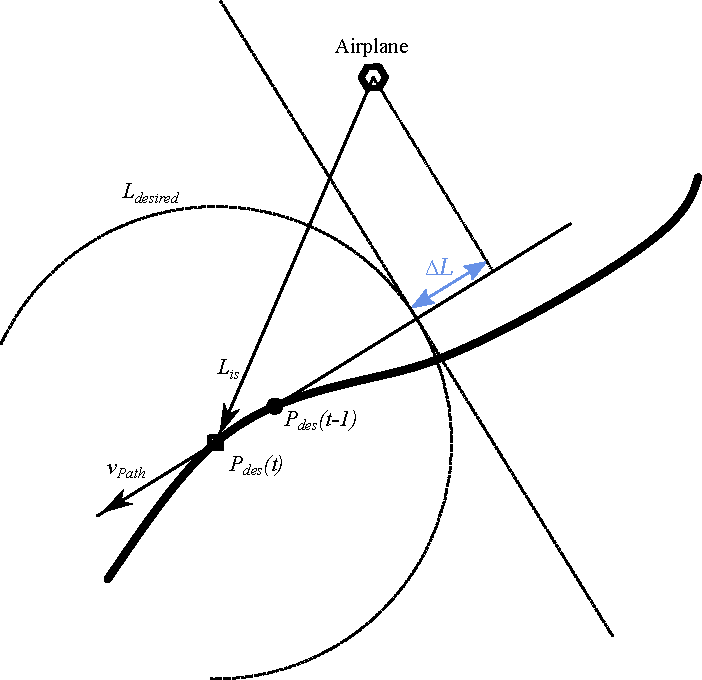
\includegraphics[width=12cm]{pictures/explanation-diagram-throttle.pdf}
  \end{center}
  \caption{Spezisfische CO\textsubscript{2-äq.}-Emissionen von Wasserstoff, über verschiedenen Prozessketten erzeugt. Unterteilung der Emissionen in die verursachenden Prozesse. Datengrundlage.}
  \label{im_spez-emissions}
\end{figure}

\noindent
Gegenüber dem Referenzfall, der Erdgas-Dampfreformierung, \cite[S.~2089]{Felgenhauer.2015}\cite{Cao.2015}


% Textende
%----------------------------------------------------------------
%----------------------------------------------------------------
% Anhang

\newpage

\begin{appendix}
%\renewcommand{\refname}{A}
\section{Appendix}

\bigskip



% Literatur
% ===========================================
\subsection{References}

\begin{flushleft}
\renewcommand{\refname}{}
\singlespacing
%\bibliography{references}
{\def\section*#1{}\bibliography{references}}
\end{flushleft}

%\newpage


\bigskip

% Abbildungsverzeichnis
% ===========================================
\subsection{List of Figures}

\renewcommand{\listfigurename}{}
%\listoffigures
{\def\section*#1{}\listoffigures}


\end{appendix}

\end{document}


% -------------------Bausteine--------------------------------------
	
%\begin{figure}[!b]
%  \begin{center}
%    \includegraphics[width=16cm]{../Machine-Epsilon-different-divisors.eps}
%  \end{center}
%  \caption{\small Figure caption. To get a figure to span two
%      columns, use the environment figure* rather than figure.}
%  \label{fig-label}
%\end{figure}


%\begin{enumerate}[{(\arabic{enumi})}]
%
%	\item
%			
%\end{enumerate}

%\begin{pspicture}[xAxisLabel=Auslastung,yAxisLabel=Herst.-Kosten](-0.5,0)(0.5,6.5)
%\begin{psgraph}[arrows=->,Dx=1,Dy=2](0,0)(-0.1,-0.1)(1.2,1.2){5cm}{4cm}
%	\psplot[plotpoints=200,linecolor=red]{0.075}{1}{0.2 0.1 x add div}
%\end{psgraph}
%\end{pspicture}

%\begin{figure}[ph]
%	\centering
%	\caption{Function with three different solvers for task~2.}
%	\lstinputlisting{../Solver.m}
%	\label{Code-Solver}
%\end{figure}

	
%\section{Literature}
%
%\renewcommand{\refname}{}
%
%\begin{flushleft}
%
%\singlespacing
%\bibliography{references}
%
%\end{flushleft}

%\begin{figure}[ph]
%	\centering
%	\subfloat[Forward Euler]{
%		\includegraphics[width=7.5cm]{../02-FE.eps}
%	}
%	\hfill
%	\subfloat[Symplectic Euler]{
%		\includegraphics[width=7.5cm]{../02-SE.eps}
%	}
%	\\
%	\centering
%	\subfloat[Stormer-Verlet]{
%		\includegraphics[width=7.5cm]{../02-SV.eps}
%	}
%	\hfill
%	\subfloat[Monat November]{
%		\includegraphics[width=7.5cm]{../02-err.eps}
%	}
%	\hfill
%	\caption{Solutions of the computed methods in task~2.}
%	\label{02}
%\end{figure}

%\renewcommand{\arraystretch}{1.4}
%\begin{table}[ht]
%\caption{Simulierte Szenarien.}
%\centering
%\begin{tabular}{R{5cm}|cc}
%\toprule 
%\textbf{Größe} & \textbf{Formelzeichen} & \textbf{Einheit} \\
%\midrule
%\textbf{Strahlungsfluss} & $\Phi_e$ & $\SI{}{\watt}$ \\
%\textbf{Bestrahlungsstärke} & $E_e = \frac{\mathrm d \Phi_e}{\mathrm d A}$ & $\SI{}{\watt \per \square \meter}$ \\
%\textbf{Lichtstrom} & $\Phi$ & $\SI{}{\lumen}$ \\
%\textbf{Beleuchtungsstärke} & $L = \frac{\mathrm d \Phi}{\mathrm d A}$ & $\SI{}{\lux} = \SI{}{\lumen \per \square \meter}$ \\
%\textbf{Lichtausbeute} & $K = \frac{\Phi}{P}$ & $\SI{}{\lumen \per \watt}$ \\
%\bottomrule 
%\end{tabular}
%\label{tab:groessen-einheiten}
%\end{table}
%\renewcommand{\arraystretch}{1.0}